

\section{循环神经网络 }\label{ux5faaux73afux795eux7ecfux7f51ux7edc}

\subsection{介绍 }\label{ux4ecbux7ecd}

可以在
\href{http://colah.github.io/posts/2015-08-Understanding-LSTMs/}{this
great article} 查看循环神经网络(RNN)以及 LSTM 的介绍。

\subsection{语言模型 }\label{ux8bedux8a00ux6a21ux578b}

此教程将展示如何在高难度的语言模型中训练循环神经网络。该问题的目标是获得一个能确定语句概率的概率模型。为了做到这一点,通过之前已经给出的词语来预测后面的词语。我们将使用
PTB(Penn Tree Bank)
数据集,这是一种常用来衡量模型的基准,同时它比较小而且训练起来相对快速。

语言模型是很多有趣难题的关键所在,比如语音识别,机器翻译,图像字幕等。它很有意思--可以参看
\href{http://karpathy.github.io/2015/05/21/rnn-effectiveness/}{here}。

本教程的目的是重现 \href{http://arxiv.org/abs/1409.2329}{Zaremba et al.,
2014} 的成果,他们在 PTB 数据集上得到了很棒的结果。

\subsection{教程文件 }\label{ux6559ux7a0bux6587ux4ef6}

本教程使用的下面文件的目录是 \texttt{models/rnn/ptb}:

\begin{longtable}[c]{@{}ll@{}}
\toprule
文件 & 作用\tabularnewline
\midrule
\endhead
\texttt{ptb\_word\_lm.py} & 在 PTB
数据集上训练一个语言模型.\tabularnewline
\texttt{reader.py} & 读取数据集.\tabularnewline
\bottomrule
\end{longtable}

\subsection{下载及准备数据
}\label{ux4e0bux8f7dux53caux51c6ux5907ux6570ux636e}

本教程需要的数据在 data/ 路径下,来源于 Tomas Mikolov 网站上的 PTB
数据集\texttt{http://www.fit.vutbr.cz/\textasciitilde{}imikolov/rnnlm/simple-examples.tgz}。

该数据集已经预先处理过并且包含了全部的 10000
个不同的词语,其中包括语句结束标记符,以及标记稀有词语的特殊符号
\texttt{(\textless{}unk\textgreater{})} 。我们在 \texttt{reader.py}
中转换所有的词语,让他们各自有唯一的整型标识符,便于神经网络处理。

\subsection{模型 }\label{ux6a21ux578b}

\subsubsection{LSTM }\label{lstm}

模型的核心由一个 LSTM
单元组成,其可以在某时刻处理一个词语,以及计算语句可能的延续性的概率。网络的存储状态由一个零矢量初始化并在读取每一个词语后更新。而且,由于计算上的原因,我们将以
\texttt{batch\_size} 为最小批量来处理数据。

基础的伪代码就像下面这样:

\begin{Shaded}
\begin{Highlighting}[]
\NormalTok{lstm }\OperatorTok{=} \NormalTok{rnn_cell.BasicLSTMCell(lstm_size)}
\CommentTok{# 初始化 LSTM 存储状态.}
\NormalTok{state }\OperatorTok{=} \NormalTok{tf.zeros([batch_size, lstm.state_size])}

\NormalTok{loss }\OperatorTok{=} \FloatTok{0.0}
\ControlFlowTok{for} \NormalTok{current_batch_of_words }\OperatorTok{in} \NormalTok{words_in_dataset:}
    \CommentTok{# 每次处理一批词语后更新状态值.}
    \NormalTok{output, state }\OperatorTok{=} \NormalTok{lstm(current_batch_of_words, state)}

    \CommentTok{# LSTM 输出可用于产生下一个词语的预测}
    \NormalTok{logits }\OperatorTok{=} \NormalTok{tf.matmul(output, softmax_w) }\OperatorTok{+} \NormalTok{softmax_b}
    \NormalTok{probabilities }\OperatorTok{=} \NormalTok{tf.nn.softmax(logits)}
    \NormalTok{loss }\OperatorTok{+=} \NormalTok{loss_function(probabilities, target_words)}
\end{Highlighting}
\end{Shaded}

\subsubsection{截断反向传播
}\label{ux622aux65adux53cdux5411ux4f20ux64ad}

为使学习过程易于处理,通常的做法是将反向传播的梯度在(按时间)展开的步骤上照一个固定长度(\texttt{num\_steps})截断。
通过在一次迭代中的每个时刻上提供长度为 \texttt{num\_steps}
的输入和每次迭代完成之后反向传导,这会很容易实现。

一个简化版的用于计算图创建的截断反向传播代码:

\begin{Shaded}
\begin{Highlighting}[]
\CommentTok{# 一次给定的迭代中的输入占位符.}
\NormalTok{words }\OperatorTok{=} \NormalTok{tf.placeholder(tf.int32, [batch_size, num_steps])}

\NormalTok{lstm }\OperatorTok{=} \NormalTok{rnn_cell.BasicLSTMCell(lstm_size)}
\CommentTok{# 初始化 LSTM 存储状态.}
\NormalTok{initial_state }\OperatorTok{=} \NormalTok{state }\OperatorTok{=} \NormalTok{tf.zeros([batch_size, lstm.state_size])}

\ControlFlowTok{for} \NormalTok{i }\OperatorTok{in} \BuiltInTok{range}\NormalTok{(}\BuiltInTok{len}\NormalTok{(num_steps)):}
    \CommentTok{# 每处理一批词语后更新状态值.}
    \NormalTok{output, state }\OperatorTok{=} \NormalTok{lstm(words[:, i], state)}

    \CommentTok{# 其余的代码.}
    \CommentTok{# ...}

\NormalTok{final_state }\OperatorTok{=} \NormalTok{state}
\end{Highlighting}
\end{Shaded}

下面展现如何实现迭代整个数据集:

\begin{Shaded}
\begin{Highlighting}[]
\CommentTok{# 一个 numpy 数组,保存每一批词语之后的 LSTM 状态.}
\NormalTok{numpy_state }\OperatorTok{=} \NormalTok{initial_state.}\BuiltInTok{eval}\NormalTok{()}
\NormalTok{total_loss }\OperatorTok{=} \FloatTok{0.0}
\ControlFlowTok{for} \NormalTok{current_batch_of_words }\OperatorTok{in} \NormalTok{words_in_dataset:}
    \NormalTok{numpy_state, current_loss }\OperatorTok{=} \NormalTok{session.run([final_state, loss],}
        \CommentTok{# 通过上一次迭代结果初始化 LSTM 状态.}
        \NormalTok{feed_dict}\OperatorTok{=}\NormalTok{\{initial_state: numpy_state, words: current_batch_of_words\})}
    \NormalTok{total_loss }\OperatorTok{+=} \NormalTok{current_loss}
\end{Highlighting}
\end{Shaded}

\subsubsection{输入 }\label{ux8f93ux5165}

在输入 LSTM 前,词语 ID 被嵌入到了一个密集的表示中(查看
\href{tensorflow-zh/SOURCE/tutorials/word2vec/index.md}{矢量表示教程})。这种方式允许模型高效地表示词语,也便于写代码:

\begin{Shaded}
\begin{Highlighting}[]
\CommentTok{# embedding_matrix 张量的形状是: [vocabulary_size, embedding_size]}
\NormalTok{word_embeddings }\OperatorTok{=} \NormalTok{tf.nn.embedding_lookup(embedding_matrix, word_ids)}
\end{Highlighting}
\end{Shaded}

嵌入的矩阵会被随机地初始化,模型会学会通过数据分辨不同词语的意思。

\subsubsection{损失函数 }\label{ux635fux5931ux51fdux6570}

我们想使目标词语的平均负对数概率最小

\begin{figure}[htbp]
\centering
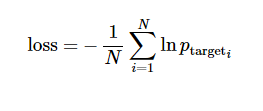
\includegraphics{../images/re.png}
\caption{}
\end{figure}

实现起来并非很难,而且函数 \texttt{sequence\_loss\_by\_example}
已经有了,可以直接使用。

论文中的典型衡量标准是每个词语的平均困惑度(perplexity),计算式为

\begin{figure}[htbp]
\centering
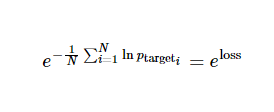
\includegraphics{../images/re1.png}
\caption{}
\end{figure}

同时我们会观察训练过程中的困惑度值(perplexity)。

\subsubsection{多个 LSTM 层堆叠
}\label{ux591aux4e2a-lstm-ux5c42ux5806ux53e0}

要想给模型更强的表达能力,可以添加多层 LSTM
来处理数据。第一层的输出作为第二层的输入,以此类推。

类 \texttt{MultiRNNCell} 可以无缝的将其实现:

\begin{Shaded}
\begin{Highlighting}[]
\NormalTok{lstm }\OperatorTok{=} \NormalTok{rnn_cell.BasicLSTMCell(lstm_size)}
\NormalTok{stacked_lstm }\OperatorTok{=} \NormalTok{rnn_cell.MultiRNNCell([lstm] }\OperatorTok{*} \NormalTok{number_of_layers)}

\NormalTok{initial_state }\OperatorTok{=} \NormalTok{state }\OperatorTok{=} \NormalTok{stacked_lstm.zero_state(batch_size, tf.float32)}
\ControlFlowTok{for} \NormalTok{i }\OperatorTok{in} \BuiltInTok{range}\NormalTok{(}\BuiltInTok{len}\NormalTok{(num_steps)):}
    \CommentTok{# 每次处理一批词语后更新状态值.}
    \NormalTok{output, state }\OperatorTok{=} \NormalTok{stacked_lstm(words[:, i], state)}

    \CommentTok{# 其余的代码.}
    \CommentTok{# ...}

\NormalTok{final_state }\OperatorTok{=} \NormalTok{state}
\end{Highlighting}
\end{Shaded}

\subsection{编译并运行代码
}\label{ux7f16ux8bd1ux5e76ux8fd0ux884cux4ee3ux7801}

首先需要构建库,在 CPU 上编译:

\begin{verbatim}
bazel build -c opt tensorflow/models/rnn/ptb:ptb_word_lm
\end{verbatim}

如果你有一个强大的 GPU,可以运行:

\begin{verbatim}
bazel build -c opt --config=cuda tensorflow/models/rnn/ptb:ptb_word_lm
\end{verbatim}

运行模型:

\begin{verbatim}
bazel-bin/tensorflow/models/rnn/ptb/ptb_word_lm \
  --data_path=/tmp/simple-examples/data/ --alsologtostderr --model small
\end{verbatim}

教程代码中有 3 个支持的模型配置参数:``small'', ``medium'' 和
``large''。它们指的是 LSTM 的大小,以及用于训练的超参数集。

模型越大,得到的结果应该更好。在测试集中 \texttt{small}
模型应该可以达到低于 120 的困惑度(perplexity),\texttt{large}
模型则是低于 80,但它可能花费数小时来训练。

\subsection{除此之外? }\label{ux9664ux6b64ux4e4bux5916}

还有几个优化模型的技巧没有提到,包括:

\begin{itemize}
\tightlist
\item
  随时间降低学习率,
\item
  LSTM 层间 dropout.
\end{itemize}

继续学习和更改代码以进一步改善模型吧。

原文:\href{http://tensorflow.org/tutorials/recurrent/index.md}{Recurrent
Neural Networks} 翻译:\href{https://github.com/Warln}{Warln}
校对:\href{https://github.com/wanghong-yang}{HongyangWang}

